% !TeX root = ../main.tex

\chapter{医学文本生成任务推断阶段的隐私保护研究}

\section{引言}

为缓解攻击者在推断阶段试图通过模型反演攻击来恢复训练隐私数据的风险,同时保持语言模型的表达能力,本章基于差分隐私机制提出两种方法。首先,本章将介绍系统模型与设计目标,引入本章的保护对象并介绍攻击者的行为。其次,本章介绍选择差分隐私的定义,并针对训练与推断阶段分别设计了选择差分隐私优化器与选择差分隐私解码算法,作为两种提供选择差分隐私的方式。随后,对前述设计的选择差分隐私优化器与选择差分隐私解码算法进行隐私性分析,以证明其满足差分隐私的定义。最后,本章通过设计实验说明这两种保护方法的优势。

\section{隐私保护系统设计与优化策略}

\subsection{系统模型}

如图 \ref{Chap5_Attatck_Model} 所示,在这种场景下,拥有隐私医学文本数据集的数据持有者通过一种训练策略得到一个针对该领域医学文本的语言模型,其通过公开推断查询的接口来提供查询服务。正常的诚实使用者将输入传给模型持有者,模型持有者通过语言模型执行推断,并将语言模型的输出返回给使用者。而调用查询接口的使用者可能会定制攻击输入前缀并通过执行多次推断服务来尝试恢复模型的隐私数据。

本节研究持有隐私数据集的数据持有者如何保障在执行推断阶段时,训练好的语言模型不会由于“记忆性”导致泄露出训练的隐私内容,即使用何种训练策略才能让模型主要关注于文本构成以及生成逻辑,而不是“记住”具体的隐私信息。因此,本节考虑两个实体,第一个是拥有隐私医学文本数据集的数据持有者,第二个是调用查询接口的使用者。



%另一方是通过模型持有者接口进行查询的使用者。多个数据持有者希望通过多个计算方提供的计算服务来协同训练模型,计算方在计算服务结束后将训练好的模型分发给各个数据持有者。

%如图\ref{Chap4_System_Info}所示,其中①表示多个数据持有者通过秘密共享算法将数据拆分成两个秘密份额分发给服务器$p_0$与服务器$p_1$。②表示在服务器$p_2$提供的相应MPC计算随机数的辅助下,服务器$p_0$与服务器$p_1$运行MPC协议来执行模型的训练过程。③表示训练结束后,服务器$p_0$与服务器$p_1$将各自的模型参数份额返还给各数据持有者。在这种场景下,我们假设有两类实体,一方是多个拥有医疗隐私数据的数据持有者,另一方是提供计算服务的三个计算方。多个数据持有者希望通过多个计算方提供的计算服务来协同训练模型,计算方在计算服务结束后将训练好的模型分发给各个数据持有者。其中作为提供计算服务的三个计算方$p_0$、$p_1$与$p_2$均具有Intel SGX,且$p_0$与$p_1$具有高性能计算GPU或者TPU(后文均以GPU指代)。

\begin{figure}[h]
	\centering
	%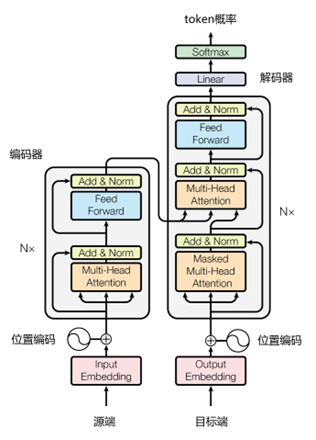
\includegraphics[width=1\textwidth]{figures/Transformer_Structure.png}sep_exeEncalveE
	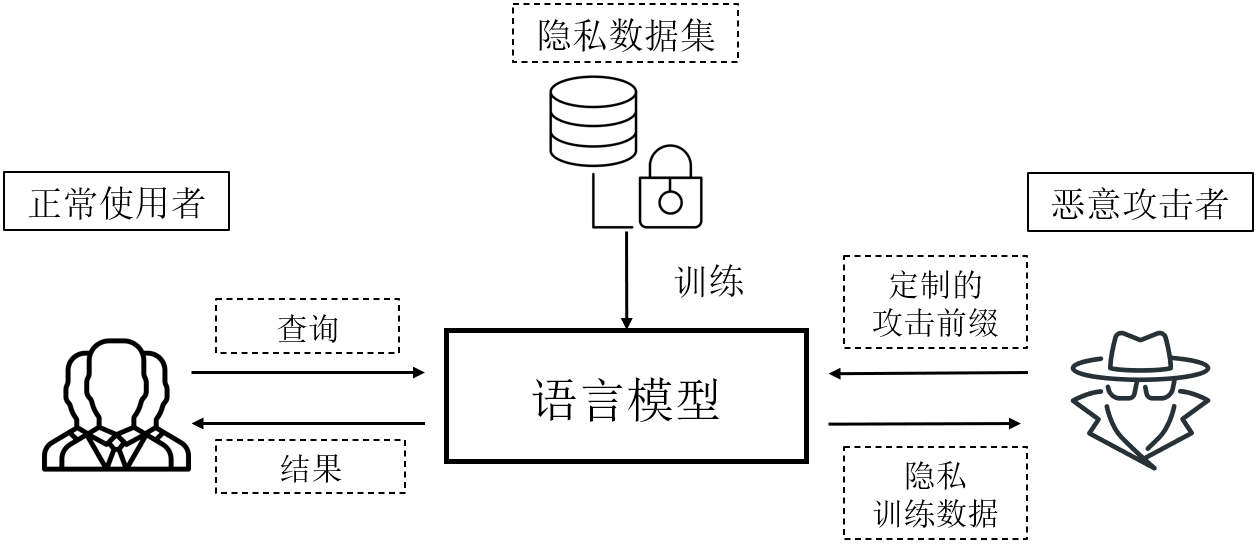
\includegraphics[width=0.7\linewidth]{figures/Chap5_Attack_Model.png}
	\caption{医学文本生成任务推断阶段的系统模型}
	\label{Chap5_Attatck_Model}
\end{figure}

\subsection{威胁模型与设计目标}

(1)威胁模型

本节对该场景下拥有隐私医学文本数据集的数据持有者的安全假设是诚实的,即它会使用真实的医学隐私训练语料通过特定的训练方式来训练模型,也称为模型持有者(后文提到的数据持有者与模型持有者在本章中都是相同的)。对于调用查询接口的使用者,本章假设其是恶意的,它可以通过定制任何攻击前缀来从模型持有者的模型中推断训练数据集的隐私信息。

(2)设计目标

\begin{itemize}
	\item [a)]
	训练阶段引入差分隐私。数据持有者通过一个隐私保护的训练算法在隐私数据上进行模型训练,推断阶段直接输出推断结果。
	\item [b)]
	推断阶段引入差分隐私。数据持有者直接使用隐私数据进行训练,推断阶段使用一个隐私保护的推断算法输出推断结果。
\end{itemize}

\subsection{训练阶段隐私保护的关联性分析}

在训练阶段的执行过程中,如果仅在训练阶段应用差分隐私算法,而不采取其他隐私保护措施,这样无法直接保护隐私信息。原因在于,即使在半诚实攻击者的场景下,以下两种情况都可能导致隐私泄露:1. 如果词嵌入(Word Embedding)也位于计算方,即使假设词表对其不可见,攻击者仍可通过接收到的输入(表示原始隐私词表上Token的序号信息)结合统计学方法和常见词表生成算法来重构隐私词表,进而恢复原始训练样本。2. 如果计算方仅处理经过词嵌入的Token,由于攻击者拥有完整模型,他们可以利用这些中间值来重构并恢复原始Token内容。因此,在训练阶段,不能直接应用第五章的方法来防止训练者窥探训练数据的隐私信息。

实际上,第四章与第五章的研究目标是不同的。第四章假设训练阶段的计算方是恶意的,旨在防止计算方获取训练隐私数据;而第五章假设推断阶段的使用者是恶意的,目的在于缓解语言模型的记忆性,从而防止模型恢复原始训练数据。这两个章节的内容是正交的,没有直接的耦合关系。因此,可以将这两种方法结合起来,这样既能防止训练时计算方窥探隐私数据,又能防止推断时使用者利用模型反演攻击恢复训练隐私数据。这样的组合方法将在保护用户隐私和数据安全方面发挥更大的作用。

\subsection{医学领域特定优化策略与评估指标} \label{medical_domain_books}

在进行医学文本生成任务的研究中,本章致力于开发特定于该领域的优化策略。为此,本章引入了一种专用的知识输入方法,该方法以开源医学教材作为主要知识来源。这些教材覆盖了医学的各个领域,包括基础医学、临床医学等,由专业的医学人员编写和审查,因此其内容准确且可靠。

这些教材包含了丰富的医学知识,包括但不限于疾病的定义、症状、诊断、治疗、预防以及医学术语等。通过将这些知识纳入模型的输入,本章的语言模型能够更深入地理解和生成与医学相关的文本,从而提高文本生成的质量。

同时,通过引入医学专业知识,本章的方法也有助于保护患者的隐私。具体来说,由于模型主要依赖于医学教材的公开知识,而非个体特定的隐私信息,因此在生成文本时,模型更少地依赖于训练数据中的隐私信息,从而降低了隐私泄露的风险。综上所述,在补充了医学教材语料后,本章的医学领域专用优化方法不仅提高了文本生成的质量,也有助于保护患者的隐私。

%如图\ref{Chap5_KnowEnhanceData}所示,本章基于在大量如翻译、新闻、论坛等中文语料上预训练的语言模型,在非隐私的医学教材语料内容上进行微调,以给模型补充补充医学背景的领域信息。随后,在涉及到患者隐私内容的医学文本数据语料上,本章将采用后续设计的选择差分隐私优化器或选择差分隐私解码算法来缓解语言模型的记忆性带来的隐私训练数据的泄露问题。

如图 \ref{Chap5_KnowEnhanceData} 所示,本章首先在诸如翻译、新闻、论坛等大量中文语料上预训练的基础上,以非隐私的医学教材语料内容进行微调,从而向模型引入医学领域的专业知识。接下来,在涉及患者隐私信息的医学文本数据上,本章采用了后续设计的选择性差分隐私优化器或选择性差分隐私解码算法。这些方法旨在缓解由于语言模型的记忆性所可能导致的隐私训练数据的泄露问题。整体上,这种策略保证了医学领域文本生成任务的高质量执行,同时也有效地维护了患者的隐私。


\begin{figure}[h]
	\centering
	%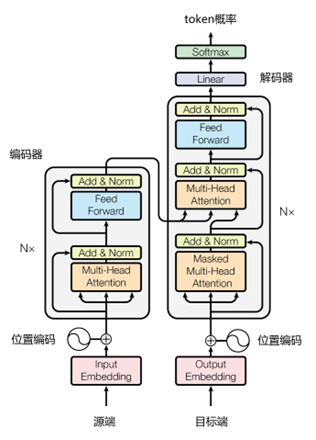
\includegraphics[width=1\textwidth]{figures/Transformer_Structure.png}sep_exeEncalveE
	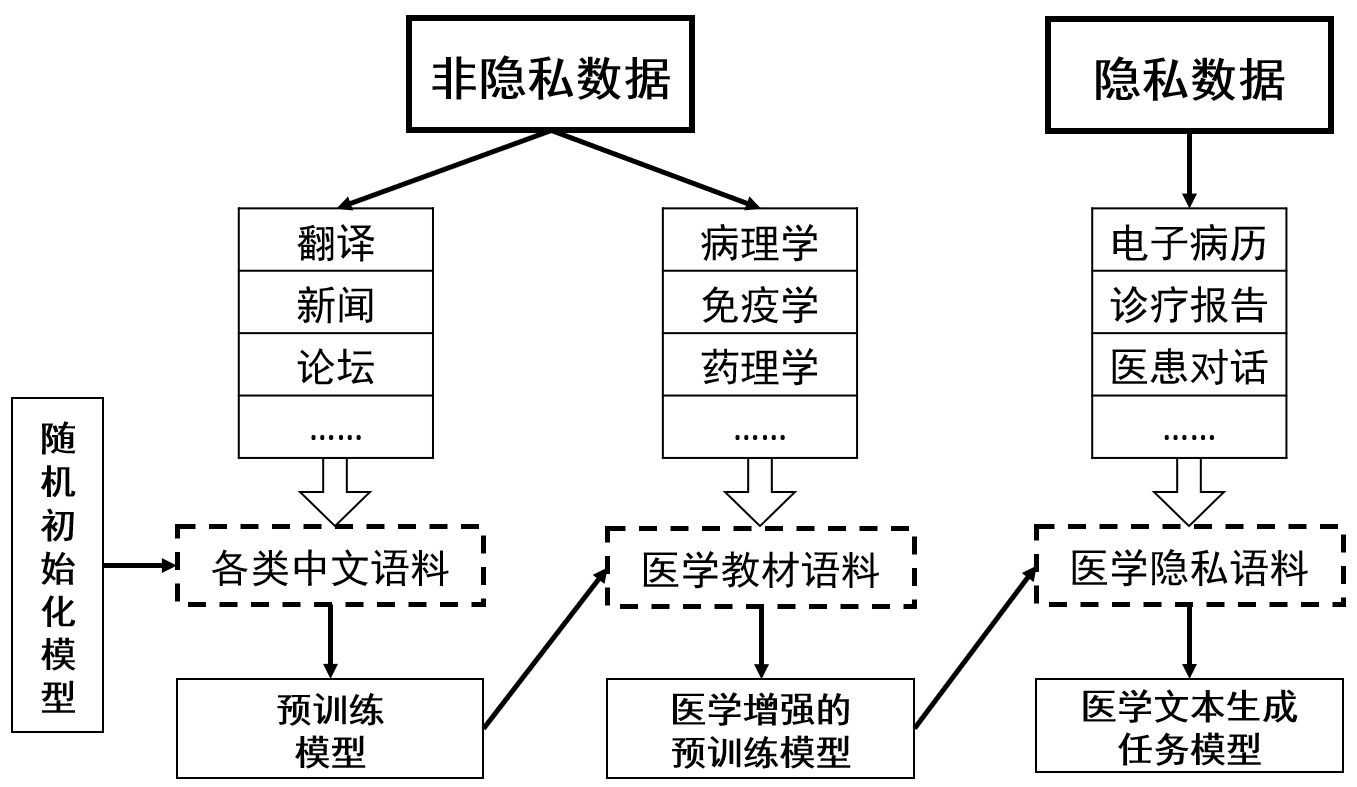
\includegraphics[width=0.8\linewidth]{figures/KnowEnhanceData.png}
	\caption{使用无隐私风险数据的微调模式}
	\label{Chap5_KnowEnhanceData}
\end{figure}



% 本节设计了一个评估生成的医学文本的科学性与准确性的困惑度指标,称为"医学文本生成的科学性"指标,并在实验中进行了评估,从而证明模型的科学性和严谨性。具体来说,如算法\ref{MedicalTermEvaluation}所示,算法首先将语言模型在医学文本上生成Logits列表。然后,我们选定医学术语token,例如“辅助检查检查脑电图检查”和“病理波、棘波、尖波、棘慢波或尖慢波”。针对这些医学术语token的Logits,我们计算它们的损失并取平均值,以此作为语言模型在生成医学术语上的表现。

在进行医学文本生成任务的过程中,对生成的文本在科学性和准确性方面有着较高的要求。为此,本章设计了一个名为"医学文本生成科学性指标"的评估方法,如算法\ref{MedicalTermEvaluation}所示。

该评估方法的输入包括一个语言模型$M$,一份医学文本$D$,一个策略函数$F$,以及一个损失函数$L$。其中,语言模型$M$被用于在医学文本上生成预测的标记分布,即Logits;策略函数$F$则用于从医学文本中识别医学术语Token,例如“双侧侧脑室显饱满”、“毛玻璃结节”、“癌胚抗原”等。

算法的核心部分是对每一篇文本$x \in D$进行处理。首先,利用语言模型$M$在$x$上生成$Logits$。然后,根据隐私筛选函数$F$选取医学术语对应的$Logits$,记为$Med\_Term\_Logits$。接下来,将这些$Logits$与语言模型对相应医学术语的预测进行比较,计算得到损失值并累加。在处理完所有的文本后,计算总损失的平均值,并将其转换为困惑度,以此作为评估指标。

这种评估方法能够反映出语言模型在生成医学术语上的准确性,从而为医学文本生成任务提供了一种可靠的评估手段,帮助研究者理解和改进模型的表现。

\begin{algorithm}[H]
	\SetAlgoLined
	\SetKwInOut{Input}{输入}
	\SetKwInOut{Output}{输出}
	
	\Input{语言模型$M$, 医学文本$D$, 策略函数$F$,损失函数$L$}
	\Output{医学文本生成的科学性指标$Evaluation\_Score$}
	
	\For{$x \in D$}{
		\# 利用语言模型在医学文本上生成$Logits$列表
		
		$Logits = M(x)$  % 利用语言模型在医学文本上生成Logits列表
		
		\# 选取医学术语对应的$Logits$
		
		$Med\_Term\_Logits = Logits[F(x)]$ % 
		
		\# 计算每个医学术语的$Loss$
		
		$Loss = Loss + L(Med\_Term\_Logits, M[F(x)])$ % 计算每个医学术语的Loss
	}

	\# 计算平均损失
	
	$Loss = Loss / |D|$
	
	\# 计算平均困惑度,作为生成能力评估值$Evaluation\_Score$
	
	$Evaluation\_Score = \exp(Loss) $ % 计算平均损失,作为生成能力评估值
	
	\caption{医学文本生成科学性指标}
	\label{MedicalTermEvaluation}
\end{algorithm}

%\section{选择差分隐私算法}

\section{基于差分隐私算法的推断结果隐私保护方案}

\subsection{选择差分隐私定义}

参考 \ref{NLP_Def} 节的介绍,考虑一个由词表$V$中的多个tokens组成的文本序列,即$x=(x_1,\dots,x_n)$,其中$x_i$为第$i$个token。语言建模的目标是,通过应用链式法则$\Pr(x)=∏_{i=1}^n \Pr(x_i |x_{<i})$构建分布的生成模型$\Pr(x)$。当用参数$\theta$评估神经网络$f$时,本节让$f_\theta(x_i|x_{<i})$表示token $x_i$的概率。通过训练最小化负对数似然函数$L(θ) = -\log ∏_{i=1}^n f_θ (x_i|x_{<i})$,来使得模型最大化训练集$W$中数据的概率。
%$$Pr(x)=∏_{i=1}^n p(x_i|x_{<i})$$
%$$L(θ)=-∑_{t=1}^{|D|} ∑_{i=1}^{n_t} log p_\theta (x_i^t |x_{<i}^t)$$

由 \ref{eps-delta-dp} 中DP的定义,若将DP直接部署在医学文本生成任务上,其对所有内容进行保护,即将所有记录视为敏感的。相关工作研究了在NLP领域使用DP的一些变体,如个性化DP\cite{DP_Personal}和onesided DP\cite{onesideDP}。然而,现有的隐私概念不允许给定记录中的不同属性具有不同的隐私级别,特别是对于隐私属性极为稀疏的NLP任务。因此,本文参考\cite{selectivedp},引入了一种新的隐私概念——选择差异隐私,即使用策略函数区分一个数据样本内部的私有和非私有属性,并保护一个数据样本的私有部分。


\begin{definition}{(策略函数)}
	策略函数$F: τ\rightarrow\{0,1\}^{n_r}$表示一个记录$r∈τ$的哪些属性是敏感的$(F(r)_i=0)$或不敏感的$(F(r)_i=1)$,其中$n_r$是$r$中的属性数量。其中,$n_r$依赖于记录,而不是一个固定的数。
	\label{metric_func}
\end{definition}

%策略函数$F: τ\rightarrow\{0,1\}^{n_r}$表示一个记录$r∈τ$的哪些属性是敏感的$(F(r)_i=0)$或不敏感的$(F(r)_i=1)$,其中$n_r$是$r$中的属性数量。其中,$n_r$依赖于记录,而不是一个固定的数。

用户可以自由定义策略函数来编码具体的隐私规定,并根据具体应用保护任何敏感属性。受保护的敏感属性类型是无限的,可以是实体(如姓名、电子邮件等)、上下文(如健康相关信息、说话风格等),等等。例如,用户可以设计一个保守的政策功能,在必要时保护选定的完整句子。策略函数的形式也是无限的,可以是神经网络、正则表达式等。

在语言建模的情况下,每个记录是一个文本序列$x$,每个属性是$x$中的一个token $x_i$, $F(x)$是一个位向量,表示哪些标记包含私有信息。本章在新的隐私概念下定义如下所示的相邻数据集。

\begin{definition}{(F-Neighbors)}
	$D, D'$是两个数据集,$F$是一个策略函数。当且仅当$∃r∈D$使得$F(r)$包含至少一个私有属性,$∃r'∈D'$ 使得$F(r)$和$F(r')$至少有一个私有属性不同,且$D'=D/\{r\}∪\{ r'\}$时,则称$D'$是$D$的相邻数据集。简记为 $D'∈N_F (D)$。
	\label{F_Neighbour}
\end{definition}

在这个定义下,包含“我的ID是123”的数据集和包含“我的ID是456”的数据集是相邻的。但带有“Hello there”的数据集和带有“Hi there”的数据集不是邻居,因为它们不包含隐私信息。

\begin{definition}{(选择差分隐私\cite{selectivedp})}
给定一个策略函数$F$。对于$∀D, D'\in N_F (D)$以及$∀T⊆R$,如果$Pr[M(D)\subset T]\leq e^\epsilon Pr[M(D')\subset T]+\delta$,则称随机算法$M:D\rightarrow R$满足$(F,\epsilon,\delta)$-Selective DP。
\label{SDP}
\end{definition}

本质上,选择性差分隐私也提供了类似于规范DP的不可区分性,但只针对记录中的敏感属性。只要保留敏感属性的隐私,选择性差分隐私并不约束非敏感属性的信息泄露。因此,选择性差分隐私在最坏的情况下(即攻击者可能知道除目标敏感属性之外的所有信息)保护敏感属性的隐私。

\subsection{针对训练阶段的选择差分隐私优化器}


%本节介绍针对训练阶段的选择差分隐私优化器。使用选择差分隐私机制的相关工作\cite{selectivedp}仅在RNN式的语言模型上实施。RNN式的模型按照token出现的顺序从前往后滑动处理,这种情况下隐私tokens与非隐私token分开处理较容易,而由于基于Transformer结构的模型所有tokens时并行处理的,因此无法直接将研究工作\cite{selectivedp}中的RNN式的处理方法用在基于Transformer的模型上。下面引入本节针对训练阶段的选择差分隐私优化器的介绍。

\begin{figure}[h]
	\centering
	%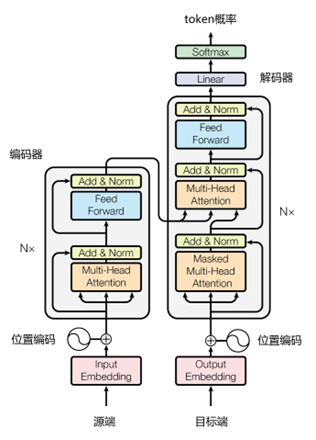
\includegraphics[width=1\textwidth]{figures/Transformer_Structure.png}
	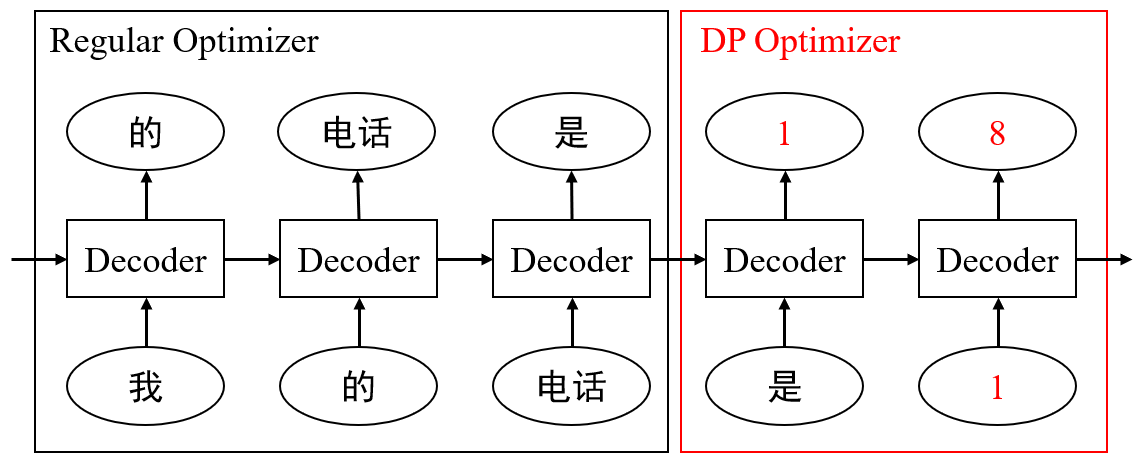
\includegraphics[width=0.7\linewidth]{figures/SDP_Optim.png}
	\caption{串行处理的选择差分隐私训练优化器}
	\label{SDP_Optim}
\end{figure}

本节介绍针对训练阶段的选择性差分隐私优化器。虽然使用选择性差分隐私机制的相关工作\cite{selectivedp}已在RNN式的语言模型上实施,但RNN式的模型按照token出现的顺序从前往后滑动处理,如图 \ref{SDP_Optim} 所示,这种情况下较容易分开处理隐私tokens与非隐私tokens。而基于Transformer结构的模型中,所有tokens是并行处理的,因此无法直接将研究工作\cite{selectivedp}中的RNN式处理方法应用于基于Transformer的模型。接下来,本部分将详细介绍针对训练阶段的选择性差分隐私优化器。

%如图\ref{SDP_Optim}和算法\ref{Algrithm_SDP_Optim}所示,用于训练基于Transformer(下文表示为Model)的语言模型,实现S-DP。其基本思路是先用策略函数确定私有属性,然后确定哪些模型变量与私有属性相关,最后对非私有变量应用常规Optimizer,对私有变量应用DP-Optimizer,如图\ref{SDP_Optim}所示。

%如算法\ref{Algrithm_SDP_Optim}所示,该优化器用于训练基于Transformer(以下简称为Model)的语言模型,实现选择差分隐私。其基本思路首先使用策略函数确定私有属性,然后确定哪些模型变量与私有属性相关,最后对非私有变量应用常规Optimizer,对私有变量应用DP-Optimizer(如图\ref{SDP_Optim}所示)。

%这里需要首先确定与私有tokens相关的变量。Model使用一个隐藏状态$h_i$对上下文进行编码,输出在词表$V$上的一个分布$p_i$。如果$x_i$是私有的,那么$h_i$、$p_i$和$L_i$都是私有的。
%
%算法\ref{Algrithm_SDP_Optim}概述了DP-Optimizer中的步骤。给定一个数据集$D$,我们应用一个策略函数$F$来获得一个比特矩阵$P=F(D)$,表示哪些Tokens是私有的。训练的每一步取一个随机batch $B$,并使用$P$将$B$拆分成一个非私有和私有元组的序列${(B_{np,i},B_{p,i})}$;然后在$B_{p,i}$上应用Optimizer (常规更新),在$B_{p,i}$上应用DP-Optimizer (隐私更新),交替进行,以更新和保护隐私。注意,除了梯度中的噪声,如果隐藏状态$h_i$是私有的,还需对其裁剪和添加噪声。这是因为在LM中,如果$x_i$是私有的,那么$h_i$也包含私有信息(如图\ref{SDP_Optim}所示),并且直接传递给下一个常规更新步骤,无法被梯度中的噪声保护。所以在$h_i$中加入噪声来保护隐私信息是很重要的。由于DP-Optimizer对梯度增加了噪声,用于计算损失的$L$和$p_i$被梯度中的噪声保护。这样一来,所有的私有变量都得到了保护。

%算法\ref{Algrithm_SDP_Optim}概述了DP-Optimizer中的步骤。在选择性差分隐私优化器的实现中,本算法针对Transformer模型中的单一解码器架构,开发了一种新的训练协议。首先,通过引入策略函数$F$,本算法将输入的训练批样本$B$映射到一个隐私矩阵$M_p$,其中$M_p$指示了哪些tokens是私有信息。在每个训练批样本中,本算法对应用了Token Embedding和Encoder的输出进行噪声注入。如果某个token的输出$E_p$与隐私矩阵$M_p$中的项对应,我们就在其上添加高斯噪声,同时还执行L2范数的裁剪以满足差分隐私的有界性需求。
%
%接下来,算法对训练批样本进行传统的前向传播,输出逻辑值向量$Logits$。然后,算法根据隐私矩阵$M_p$,对模型参数进行选择性的差分隐私优化。对于非私有的tokens,本算法简单地计算损失函数$L(\theta)$的梯度并进行参数更新。然而,对于私有的tokens,算法首先计算损失函数的梯度$g(k)$,对其进行L2范数裁剪,然后再加上与隐私级别成比例的高斯噪声。最后,算法使用含噪声的梯度进行模型参数的更新。这样,所有的私有变量都得到了保护,从而实现了在训练神经网络模型时对个体隐私的保护。

算法 \ref{Algrithm_SDP_Optim} 概述了选择性差分隐私优化器中的步骤。本算法独特地针对了Transformer模型中的单一解码器架构,并开发了一种新的训练协议。这与常规的RNN模型从前向后的处理方式有着显著的区别。在选择性差分隐私优化器的实现中,该算法在Word Embedding阶段加入噪声,然后并行处理整个句子,而不是逐字处理。这是基于Transformer模型的自然特性,即其并行处理能力和对顺序无关性。

首先,通过引入策略函数$F$,本算法将输入的训练批样本$B$映射到一个隐私矩阵$M_p$,其中$M_p$指示了哪些tokens是私有信息。对于每个训练批样本,本算法对Word Embedding阶段以及Encoder输出阶段应用了噪声注入。具体来说,如果某个token的输出$E_p$与隐私矩阵$M_p$中的项对应,就在其上添加高斯噪声,同时还执行L2范数的裁剪以满足差分隐私的有界性需求。

接下来,算法对训练批样本进行传统的前向传播,输出逻辑值向量$Logits$。然后,算法根据隐私矩阵$M_p$,对模型参数进行选择性的差分隐私优化。对于非私有的tokens,本算法简单地计算损失函数$L(\theta)$的梯度并进行参数更新。然而,对于私有的tokens,算法首先计算损失函数的梯度$g(k)$,对其进行L2范数裁剪,然后再加上与隐私级别成比例的高斯噪声。最后,算法使用含噪声的梯度进行模型参数的更新。这样,所有的私有变量都得到了保护,从而实现了在训练神经网络模型时对个体隐私的保护。



%\begin{algorithm}[H]
%	% \renewcommand{\thealgocf}{}     %<---细节与重点
%	\SetAlgoLined
%	\SetKwInOut{Input}{输入}
%	\SetKwInOut{Output}{输出}
%	\Input{$N$个样本的数据集$D$,策略函数$F$,隐私矩阵$P=F(D)$,最大序列长度$K$,损失函数$L(\theta)$,超参数:学习率$\eta$、噪声指数$\sigma$、梯度裁剪上界$C$、批大小$B$,模型参数$\rm Model=\{Token\_Embedding, Encoder, Vocab\_Projection\}$}
%	
%	\Output{模型经过一轮训练更新后的参数$\rm Model$}
%	
%	\For{$j = 1, 2, \dots, B$}{
%		
%		%记Batch\_input[i]中第$j$个句子的内容Batch\_input[i][j]为Sen
%		
%		\For{$k = 1, 2, \dots, len(Sen)$}{
%			记$Batch\_input[i]$的第$j$个句子$Batch\_input[i][j]$为$x$
%			
%			使用隐私矩阵$P=F(input)$将$B$中的数据拆分成非隐私元组与隐私元组:$\{(M_{np}, M_{p})\}$
%			
%			$ E = \text{Token\_Embedding}(x)$
%			
%			$ Out\_E = \text{Encoder}(E)$
%			
%			\For{$x_k\in M_{p}$}{
%
%				$Out\_E_{p}\leftarrow Out\_E_{p} / max(1, \frac{\Vert Out\_E \Vert_2}{C})$
%
%				$Out\_E_{p} \leftarrow Out\_E_{p} + \sigma C\cdot N(0, I)$
%			}
%
%			$Logits[j] = \text{Vocab\_Projection}(Out\_E[-1])$
%			
%		}
%		
%		\For{$k = 1, 2, \dots, len(Sen) - 1$}{			
%			%$Loss[k] = L(Logits[k], x[k + 1])$
%			\If{$ k\in M_{p}$}{
%			%\For{$\rm k\in M_{p}$}
%				$g(k) \leftarrow \nabla_\theta L(\theta, Logits[k], x[k + 1])$
%				
%				$g(k) \leftarrow g(k) / max(1, \frac{\Vert g \Vert_2}{C})$
%
%				$g(k) \leftarrow \frac{1}{|M_{p}|} (\sum_j g(k) + \sigma C\cdot N(0, I))$
%
%				$\theta \leftarrow \theta - \eta g(k)$		
%			}
%			\Else{$\theta \leftarrow \theta - \eta \nabla_\theta L(\theta)$	}		
%		}
%	}
%	
%	\caption{选择差分隐私优化器}
%	\label{Algrithm_SDP_Optim}
%\end{algorithm}

\begin{algorithm}[H]
	% \renewcommand{\thealgocf}{}     %<---细节与重点
	\SetAlgoLined
	\SetKwInOut{Input}{输入}
	\SetKwInOut{Output}{输出}
	\Input{训练批样本$B$,策略函数$F$,隐私矩阵$M_p=F(B)$,损失函数$L(\theta)$,超参数:学习率$\eta$、噪声指数$\sigma$、梯度裁剪上界$C$、批大小$B$,模型参数$\rm Model=\{Token\_Embedding, Encoder, Vocab\_Projection\}$}
	
	\Output{更新后的模型参数$\rm Model$}
	
	\For{$x \in B$}{
		$ E = \text{Token\_Embedding}(x)$
		
		\For{$x_k\in M_{p}$}{
			
			$E_{p}=E[x_k]$
			
			$E_{p}\leftarrow E_{p} / max(1, \frac{\Vert E \Vert_2}{C})$
			
			$E_{p} \leftarrow E_{p} + \sigma C\cdot N(0, I)$
		}
		
		$ Out\_E = \text{Encoder}(E)$
	
		$Logits = \text{Vocab\_Projection}(Out\_E[1:-1])$
	}

	\For{$x \in B$}{
				
		\If{$ x_k\in M_{p}$}{

			$g(x_k) \leftarrow \nabla_\theta L(\theta, Logits[x_k], x_k)$
								
			$g(x_k) \leftarrow g(x_k) / max(1, \frac{\Vert g \Vert_2}{C})$
				
			$g(x_k) \leftarrow \frac{1}{|M_{p}|} (\sum_j g(x_k) + \sigma C\cdot N(0, I))$
				
			$\theta \leftarrow \theta - \eta g(x_k)$		
		}
		\Else{
			
			$\theta \leftarrow \theta - \eta \nabla_\theta L(\theta)$
		}		
	}
	
	\caption{并行处理的选择差分隐私优化器}
	\label{Algrithm_SDP_Optim}
\end{algorithm}


\subsection{针对推断阶段的选择差分隐私解码算法}

如图 \ref{Chap5_PDP_Decode} 与算法 \ref{Algrithm_SDP_Decoding} 概述了针对推断阶段的解码算法。由于该场景下训练阶段使用原始包含隐私内容的数据集进行训练,在推断阶段时,为保护隐私内容,需要对生成结果进行处理。具体来说,在生成输出的过程中,使用策略函数$F$对已生成的内容与当前模型输出的下一个Token进行判断,若属于隐私内容,则对Logits进行裁剪并加上由隐私预算与裁剪上界确定的高斯噪声,并重新经过分词器解码得到新的Token。

\begin{figure}[h]
	\centering
	%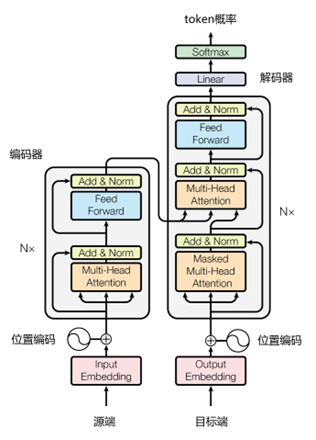
\includegraphics[width=1\textwidth]{figures/Transformer_Structure.png}
	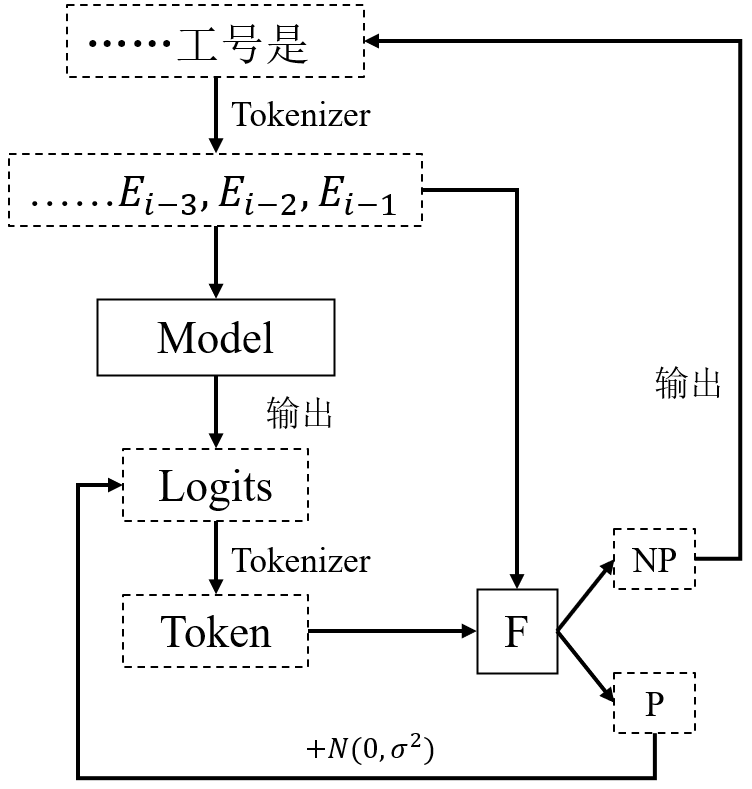
\includegraphics[width=0.44\linewidth]{figures/Chap5_PDP_Decode.png}
	\caption{选择差分隐私解码算法}
	\label{Chap5_PDP_Decode}
\end{figure}

%这里对于Logits的处理需要重点关注。由于最终确定下一个Token位于词表上的哪一个的时候使用的是Softmax(Logits),而Softmax函数不改变最大值的位置,因此选择argmax(Softmax(Logits))与argmax(Logits)的结果相同。由于Softmax($\cdot$)$\in (0, 1)$,即Softmax(Logits)输出的结果在0到1之间,有界,然而Logits$\in R$无界,因此需要对Logits进行处理以满足有界的差分隐私全局敏感度。这里,本节使用归一化处理将Logits限制在0到1之间。具体来说,对于$l_i \in Logits$,$l_i'=\frac{l_i-l_min}{l_max-l_min}$。这样,$l_i'$满足$l_i'\in [0,1]$,即这里全局敏感度$C=1$。

在文本生成任务中,生成的下一个单词通常是通过计算Logits值,再使用Softmax函数将Logits转化为概率分布来确定的。在差分隐私的场景下,需要对Logits进行处理以满足有界的全局敏感度。具体地,本章采用归一化处理将Logits限制在0到1之间。对于每个Logit $l_i$,计算其归一化后的值 $l_i' = \frac{l_i - l_{\text{min}}}{l_{\text{max}} - l_{\text{min}}}$,其中 $l_{\text{min}}$ 和 $l_{\text{max}}$ 分别是Logits中的最小值和最大值。这样,归一化后的Logits $l_i'$ 满足 $l_i' \in [0, 1]$,即全局敏感度 $C=1$。

需要注意的是,在使用Softmax函数来确定下一个单词时,Softmax函数不改变最大值的位置,因此选择 argmax(Softmax(Logits)) 与 argmax(Logits) 的结果相同。由于 Softmax(Logits) 的输出结果在 (0, 1) 范围内,即有界,而 Logits 的取值范围是实数集,即无界,因此需要对 Logits 进行归一化处理以满足有界的差分隐私全局敏感度。



\begin{algorithm}[H]
	% \renewcommand{\thealgocf}{}     %<---细节与重点
	\SetAlgoLined
	\SetKwInOut{Input}{输入}
	\SetKwInOut{Output}{输出}
	\Input{输入解码的前缀$P$,策略函数$F$,裁剪上界$C$、组大小$L$,模型$\rm Model$,词表$V$,分词器Tokenizer($\cdot$)}
	
	\Output{输入解码的前缀为$Prefix$时,模型的输出结果$Output$}
	
	\# 将当前生成结果记为CS,初始赋值为输入前缀
	
	$CS = P$
	
%	\# PS为策略函数输出的隐私分类,初始赋值为False,即认为所有输入前缀均非敏感
%	
%	PS = [False] * len(P)
	
	\# 模型输出预测下一个Token的Logits
	
	$NT\_Logits = \text{Model}(CS)$
	
	\# Logits确定最大概率的index,并由分词器解码成输出字符
	
	$NT = \text{Tokenizer}(\text{argmax}(\text{Softmax}(NT\_Logits)))$
	
	\# 若输出<EOS>符号终止流程
	
	\While{$NT!=\rm<EOS>$}{
		
		\# 若已生成内容与当前预测的下一个Token在策略函数$F$下是隐私内容,则需要加噪处理
		
		\If{$F(CS, NT) == True$}{
			\# 对Logits进行裁剪
			$NT\_Logits \leftarrow NT\_Logits / max(1, \frac{\Vert NT\_Logits \Vert_2}{C})$
			
			\# 加噪
			
			$NT\_Logits \leftarrow NT\_Logits + \sigma C\cdot N(0, I)$
			
			\# 在加噪的Logists下重新生成Token
			
			$NT = \text{Tokenizer}(\text{argmax}(\text{Softmax}(NT\_Logits)))$
		}
		
		\# 将新Token加入当前生成结果CS中
		
		$CS = CS + NT$
		
		\# 继续预测下一个Token的Logits
		
		$NT\_Logits = \text{Model}(CS)$
		
		\# 由分词器对index进行解码
		
		$NT = \text{Tokenizer}(\text{argmax}(\text{Softmax}(NT\_Logits)))$
	}

	
	\caption{选择差分隐私解码算法}
	\label{Algrithm_SDP_Decoding}
\end{algorithm}



\section{安全性分析}

本部分给出算法 \ref{Algrithm_SDP_Optim} 的隐私分析。

%矩审计(Moments Account,MA)\cite{DLDP}相较于

对于任何给定的数据集$D$,设$D_{i,j}$表示第$i$条记录的第$j$个属性。本章将梯度更新和隐藏状态抽象为以训练数据$x$和辅助信息$w$为输入的查询函数$f(x, w)$。本章引入$w$作为$f$的额外输入,以模拟梯度更新和隐藏状态对前几轮模型参数的依赖关系。具体而言,本章在数据集上定义以下两种类型的查询。
\begin{itemize}
	\item [$\cdot$]类型1:函数$f$的输入只包含策略函数$F$判定为隐私信息的查询$x$
	\item [$\cdot$]类型2:函数$f$的输入只包含策略函数$F$判定为非隐私信息的查询$x$

\end{itemize}


由于算法 \ref{Algrithm_SDP_Optim} 仅针对隐私信息进行保护,因此类型2的非隐私查询不会造成隐私损失。

下面的定理表明,如果一个类型1查询具有输出有界的属性,那么对于任意的输入,在查询中添加高斯噪声可以提供差分隐私保障。由于在策略函数$F$下的近邻数据集的非敏感部分可能是不同的,因此需要分析在任意辅助输入下的DP保证。

\begin{definition}
	(隐私损失\cite{Algorithmic_Foundations_of_DP})对于任意近邻数据集$D$与$D'$,独立的辅助输入$w$,算法$M$的输出结果为$y$,定义隐私损失如下:
	\begin{equation}
		L(y;M,w,D,D')=\ln\frac{\Pr[M(w,D)=y]}{\Pr[M(w,D')=y]}\text{。}
	\end{equation}
\end{definition}

\begin{theorem} \label{guassian_mechanism}
	记$\Delta_2f=max_{\{D,D'\}}||f(D)-f(D')||_2$函数$f$的敏感度,$N(0,\sigma^2)$为由参数$\sigma$控制的高斯分布,对于$c^2>2ln(1.25/\delta)$,具有$\delta\geq c\Delta_2f/\epsilon$的高斯机制满足$(\epsilon,\delta)$-差分隐私。
\end{theorem}

\begin{proof}
	对于数据集$D$与函数$f$,高斯机制计算结果为$f(D)+N(0,\sigma^2)$,其中$N(0,\sigma^2)$为均值为0,标准差为$\sigma$的高斯分布。考虑如下表达式:
	\begin{equation}
		\lvert \ln\frac{e^{(-1/2\sigma^2)x^2}}{e^{(-1/2\sigma^2)(x+\Delta f)^2}}\rvert\text{,}
	\end{equation}
	这个式子是隐私损失的绝对值。
	假设数据集是$D$,为证明高斯机制满足$(\epsilon,\delta)$-差分隐私,则需观察在$D$下与在其近邻数据集$D'$下,输出结果非常不同时的概率。上式中的分子描述了当数据集为$D$时看到$f(D)+x$的概率,分母对应的是当数据集为$D'$时看到这个相同值的概率,即该分式为非负的概率的比值,但其对数可能是负的。为方便起见,本部分研究隐私预算的绝对值。
	\begin{equation}
		\begin{aligned}
			\lvert \ln\frac{e^{(-1/2\sigma^2)x^2}}{e^{(-1/2\sigma^2)(x+\Delta f)^2}}\rvert
			& = \lvert \ln e^{(-1/2\sigma^2)[x^2-(x+\Delta f)^2]}\rvert\\
			& = \lvert -\frac{1}{2\sigma^2}[x^2-(x+\Delta f)^2]\rvert\\
			& = \lvert -\frac{1}{2\sigma^2}[x^2-(x^2+2x\Delta f+\Delta f^2)]\rvert\\
			& = \lvert \frac{1}{2\sigma^2}(2x\Delta f+\Delta f^2)\rvert\\\text{。}
		\end{aligned}
	\end{equation}
	上式结果在$x < \sigma^2\epsilon/\Delta f - \Delta f /2$时可以由$\epsilon$约束。为确保隐私损失在$1-\delta$的概率下不超过隐私预算$\epsilon$,需要
	$$\Pr[|x|\geq \sigma^2\epsilon/\Delta f - \Delta f /2] < \delta\text{。}\text{。}$$
	去掉绝对值,即意味着需要找到$\sigma$使得
	$$\Pr[x\geq \sigma^2\epsilon/\Delta f - \Delta f /2] < \delta / 2\text{。}$$
	假设$\epsilon \leq 1\leq \Delta f$,利用
	$$\Pr[x>t]\leq \frac{\sigma}{\sqrt{2\pi}}e^{-t^2/2\sigma^2}\text{。}$$
	即需要
	\begin{equation}
		\begin{aligned}
			\frac{\sigma}{\sqrt{2\pi}}\frac{1}{t}e^{-t^2/2\sigma^2} < \delta / 2
			& \iff \sigma\frac{1}{t}e^{-t^2/2\sigma^2} < \sqrt{2\pi}\delta / 2\\
			& \iff \frac{t}{\sigma}e^{t^2/2\sigma^2} > 2/\sqrt{2\pi}\delta\\
			& \iff \ln(t/\sigma)+t^2/2\sigma^2>\ln(2/\sqrt{2\pi}\delta)\text{。}\notag\\ 
		\end{aligned}
	\end{equation}
	令$t=\sigma^2\epsilon/\Delta f-\Delta f/2$,即有
	$$\ln((\sigma^2\epsilon/\Delta f-\Delta f/2)/\sigma+(\sigma^2\epsilon/\Delta f-\Delta f/2)^2/2\sigma^2>\ln(2/\sqrt{2\pi}\delta))$$
	$$=\ln(\sqrt{\frac{2}{\pi}}\frac{1}{\delta})\text{。}$$
	
	记$\sigma=c\Delta f/\epsilon$,为了约束$c$,记找到第一项非负的条件。
	\begin{equation}
		\begin{aligned}
			\frac{1}{\sigma}(\sigma^2\frac{\epsilon}{\Delta f}-\frac{\Delta f}{2})
			& = \frac{1}{\sigma}[(c^2\frac{(\Delta f)^2}{\epsilon^2})\frac{\epsilon}{\Delta f}-\frac{\Delta f}{2}]\\
			& = \frac{1}{\sigma}[c^2\frac{\Delta f}{\epsilon}-\frac{\Delta f}{2}]\\
			& = \frac{\epsilon}{c\Delta f}[c^2\frac{\Delta f}{\epsilon}-\frac{\Delta f}{2}]\\
			& = c-\frac{\epsilon}{2c}\text{。}\notag\\ 
		\end{aligned}
	\end{equation}
	由于$\epsilon\leq 1$且$c\geq 1$,即$c-\epsilon/c\geq c - 1/2$,故当$c\geq 3/2$时,$\ln(\frac{1}{\sigma}(\sigma^2\frac{\epsilon}{\Delta f}-\frac{\Delta f}{2}))>0$。接下来关注$t^2/\sigma^2$这一项。
	\begin{equation}
		\begin{aligned}
			(\frac{1}{2\sigma^2}\frac{\sigma^2\epsilon}{\Delta f}-\frac{\Delta f}{2})^2
			& = \frac{1}{2\sigma^2}[\Delta f(\frac{c^2}{\epsilon}-\frac{1}{2})]^2\\
			& = \frac{1}{2}[(\Delta f)^2(\frac{c^2}{\epsilon}-\frac{1}{2})]^2[\frac{\epsilon^2}{c^2(\Delta f)^2}]\\
			& = \frac{1}{2}(\frac{c^2}{\epsilon}-\frac{1}{2}))^2\frac{\epsilon^2}{c^2}\\
			& = \frac{1}{2}(c^2-\epsilon+\epsilon^2/4c^2)\text{。}\notag\\ 
		\end{aligned}
	\end{equation}
	由于$\epsilon\leq 1$并且$c\geq 3/2$,则$c^2-\epsilon+\epsilon^2/4c^2\geq c^2-8/9$,故仅需
	$$c^2-8/9>2\ln(\sqrt{\frac{2}{\pi}}\frac{1}{\delta})\text{。}$$
	换言之,需要
	$$c^2>2\ln(\sqrt{\frac{2}{\pi}})+2\ln(\frac{1}{\delta})+\ln(e^{8/9})=\ln(2/\pi)+\ln(e^{8/9})+2\ln(\frac{1}{\delta})\text{。}$$
	且由于$(2/\pi)e^{8/9}<1.55$,上式在$c^2>2\ln(1.25/\delta)$时成立。
	
	记$R_1=\{x\in R:|x|\leq c\Delta f/\epsilon\}$与$R_2=\{x\in R:|x|> c\Delta f/\epsilon\}$,易知$R=R_1\cup R_2$,取$S\subset R$,并记
	$$S_1=\{f(x)+x|x\in R_1\}\text{,}$$
	$$S_2=\{f(x)+x|x\in R_2\}\text{,}$$
	则有
	\begin{equation}
		\begin{aligned}
			\Pr\limits_{x\sim N(0,\sigma^2)}[f(x)+x\in S]
			& = \Pr\limits_{x\sim N(0,\sigma^2)}[f(x)+x\in S_1]\\
			& + \Pr\limits_{x\sim N(0,\sigma^2)}[f(x)+x\in S_2]\\
			& \leq \Pr\limits_{x\sim N(0,\sigma^2)}[f(x)+x\in S_1] + \delta\\
			& \leq e^\epsilon\left(\Pr\limits_{x\sim N(0,\sigma^2)}[f(y)+x\in S_1]\right) + \delta\text{。}\\
		\end{aligned}
	\end{equation}
	故高斯机制满足$(\epsilon,\delta)$-差分隐私。
	
\end{proof}

\begin{theorem}
	\label{gxw_gdp}
	假设$max_{x,w}||g(x,w)||\leq C$,对于任意的$w$,添加由$C$确定的高斯分布噪声可以保证$g$满足$(\epsilon, \delta)$-差分隐私,其中$\epsilon, \delta$取决于$C$与$\sigma$。形式化来说,对于近邻数据集$(x, x')$以及任意的$(w, w')$,有
	$$\frac{P[g(x,w) + \Delta = r]}{P[g(x',w') + \Delta = r]}\leq e^\epsilon \quad w.p.\quad1-\delta\text{。}$$
\end{theorem}

算法 \ref{Algrithm_SDP_Optim} 中对于梯度信息进行了裁剪,即满足有界性,由引理 \ref{guassian_mechanism} 知,定理\ref{gxw_gdp}成立。同样的,算法 \ref{Algrithm_SDP_Decoding} 中对于Logits信息进行了裁剪,即满足有界性,由引理 \ref{guassian_mechanism} 知,定理 \ref{gxw_gdp} 成立。算法 \ref{Algrithm_SDP_Optim} 对于非隐私内容$B_{np,i}$的更新属于类型2,这样的更新不会导致使用更多的隐私预算。对于隐私内容的更新(包括梯度与隐藏状态$Hidden$)属于类型1,称其加上满足引理 \ref{guassian_mechanism} 中的高斯噪声后的数据为“模糊的”类1查询。算法 \ref{Algrithm_SDP_Optim} 中的数据实际上由类型2与“模糊的”类型1构成。算法 \ref{Algrithm_SDP_Decoding} 中的数据同样由类型2与“模糊的”类型1构成。下面论证这样的组合满足$(\epsilon, \delta)$-差分隐私。

\begin{theorem}
	\label{gxw_gdp}
	记是$f$为由$k$个查询$\{f_1,\cdots f_k\}$构成的整体,其中$f_i$属于类型1或“模糊的”类型2。给定策略函数$F$,记$f_{np}$为类型2,$f_p$为“模糊的”类型1。那么如果$f_p$满足$(\epsilon, \delta)$-差分隐私,则$f$满足$(F,ϵ,δ)$-Selective DP。
\end{theorem}

%\begin{proof}
%	考虑在策略函数$F$下的近邻数据集$x$与$x'$,记$x_i$与$x_i'$是数据$f_i$中的子集。若$f_i$属于“模糊的”类型1的,则$x_i$只包含隐私内容,反之若$f_i$属于类型2,$x_i$只包含非隐私内容。由于$x$与$x'$是策略函数$F$下的紧邻数据集,即$f_i$属于“模糊的”类型1。对于$f$的一个输出$\{y_1,\cdots y_k\}$,有
%	\begin{align}
%		&\frac{P[f_1(x_1,w_1)=y_1,\cdots,f_1(x_k,w_k)=y_k]}{P[f_1(x_1',w_1')=y_1',\cdots,f_1(x_k',w_k')=y_k']}\notag\\
%		&=\prod_{f_i\in f_p}\frac{f_i(x_i,w_i)=y_i}{f_i(x_i',w_i')=y_i'} \label{chap5pfline2}\\
%		&\leq e^\epsilon \quad w.p.\quad1-\delta \label{chap5pfline3}
%	\end{align}
%	式\ref{chap5pfline2}是由于$f_{np}$不涉及隐私内容并且每一个token的隐层表示与其对损失函数的贡献是独立的。式\ref{chap5pfline3}中的不等式是因为$f_p$满足$(\epsilon, \delta)$-差分隐私的假设。
%\end{proof}


\begin{proof}
	考虑在策略函数 $F$ 下的近邻数据集 $x$ 与 $x'$,记 $x_i$ 与 $x_i'$ 是数据 $f_i$ 中的子集。若 $f_i$ 属于 "模糊的" 类型 1,则 $x_i$ 只包含隐私内容;反之若 $f_i$ 属于类型 2,$x_i$ 只包含非隐私内容。由于 $x$ 与 $x'$ 是策略函数 $F$ 下的紧邻数据集,即 $f_i$ 属于 "模糊的" 类型 1。对于 $f$ 的一个输出 ${y_1,\cdots y_k}$,有

	\begin{align}
		&\frac{P[f_1(x_1,w_1)=y_1,\cdots,f_1(x_k,w_k)=y_k]}{P[f_1(x_1',w_1')=y_1',\cdots,f_1(x_k',w_k')=y_k']}\notag\\
		&=\prod_{f_i\in f_p}\frac{f_i(x_i,w_i)=y_i}{f_i(x_i',w_i')=y_i'} \label{proof_line2}\\
		&\leq e^\epsilon \quad w.p.\quad1-\delta \text{。}\label{proof_line3}
	\end{align}
	
	式 \ref{proof_line2} 是由于 $f_{np}$ 不涉及隐私内容,并且每一个 token 的隐层表示与其对损失函数的贡献是独立的。式 \ref{proof_line3} 中的不等式是因为 $f_p$ 满足 $(\epsilon, \delta)$-差分隐私的假设。
\end{proof}

通过这个证明,可以得出结论:在给定策略函数 $F$ 的情况下,如果 "模糊的" 类型 1 查询 $f_p$ 满足 $(\epsilon, \delta)$-差分隐私,则整个查询 $f$ 满足 $(F, \epsilon, \delta)$-选择差分隐私。这意味着,通过在梯度上添加高斯噪声,可以确保模型训练过程满足选择差分隐私的要求,从而保护数据集中个体的隐私。

\section{实验评估}

\subsection{攻击方式}

本章执行两种类型的攻击: “诱饵”插入攻击和成员推断攻击。

(1)“诱饵”插入攻击

“诱饵”(Canary)插入攻击\cite{canary}是一种针对训练数据的隐私攻击方法,为一种定量评估意外记忆风险的测试方法。攻击者在训练数据集中插入一些特制的“诱饵”数据(即Canary),这些数据通常具有特定的模式或特征,使其在整个数据集中独特而容易识别。通过将随机序列 Canary 插入训练数据集,并在此基础上训练模型。攻击者的目标是通过分析模型的输出结果,识别出模型是否泄露了这些插入的Canary数据。

在执行Canary插入攻击时,攻击者首先需要构建一些含有特定信息的诱饵数据。这些数据应该具有一定的复杂性,以便在模型生成的输出中能够辨别出其所学习到的信息。攻击者将这些诱饵数据插入到训练数据集中,并记录下与这些诱饵数据相关的标签。然后,攻击者观察模型在特定输入下的输出结果,判断模型是否泄露了插入的Canary数据。

如果模型在生成输出时泄露了Canary数据,那么攻击者可以根据这些信息推断出模型的训练数据中可能包含了这些插入的诱饵数据。从而揭示了模型对训练数据的记忆情况,进而可能导致训练数据的隐私泄露。可以通过计算插入的Canary作为一种定量指标,以衡量模型潜在的隐私风险。其中定量的评估指标定义如下。

\begin{definition}{(Canary暴露度\cite{canary})}
	给定一个Canary $s[r]$,一个参数为$\theta$的模型,随机空间$R$,$s[r]$的暴露程度是:
	$Exposure_\theta=log_2 |R|-log_2 Rank_\theta(s[r])$
	\label{Canary_Insertion}
\end{definition}

训练后,计算所有可能实例化的Canary的模型困惑度,并将其按照困惑度排序。然后根据特定Canary序列的$Rank_\theta(s[r])$和所有可候选的数量$|R|$得到Canary的暴露量。从定义来看,当Canary在所有输出的排名越靠前,则暴露的程度就越高,而rank高意味着后面$Rank_\theta(s[r])$的值越低,则$log_2 |R|-log_2 Rank_\theta(s[r])$的值越高。因此,若模型的Canary暴露度越高,则它记忆训练样本的可能性越高,即暴露程度越高。反之,若模型的Canary暴露度很低,则说明该模型更倾向于学习到模式而非具体的内容,即对训练数据的隐私保护程度较高。在本章设置中,实验显示了10个Canary中最高的Canary暴露。例如,如果一个Canary在100万个候选中排名第一,那么Canary的暴露量是19.93。如图 \ref{Chap5_CanaryInsertion} 所示,当在训练过程中插入的 Canary 为“我的单号是 \#3006……”并在之前输入确定时,将LM输出的logits按照Softmax后的$P$概率值排序,找到与Canary匹配的token的rank排名,作为攻击的度量指标。


\begin{figure}[h]
	\centering
	%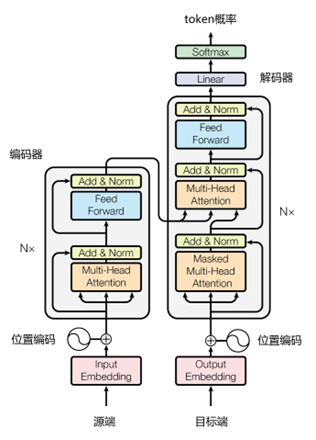
\includegraphics[width=1\textwidth]{figures/Transformer_Structure.png}
	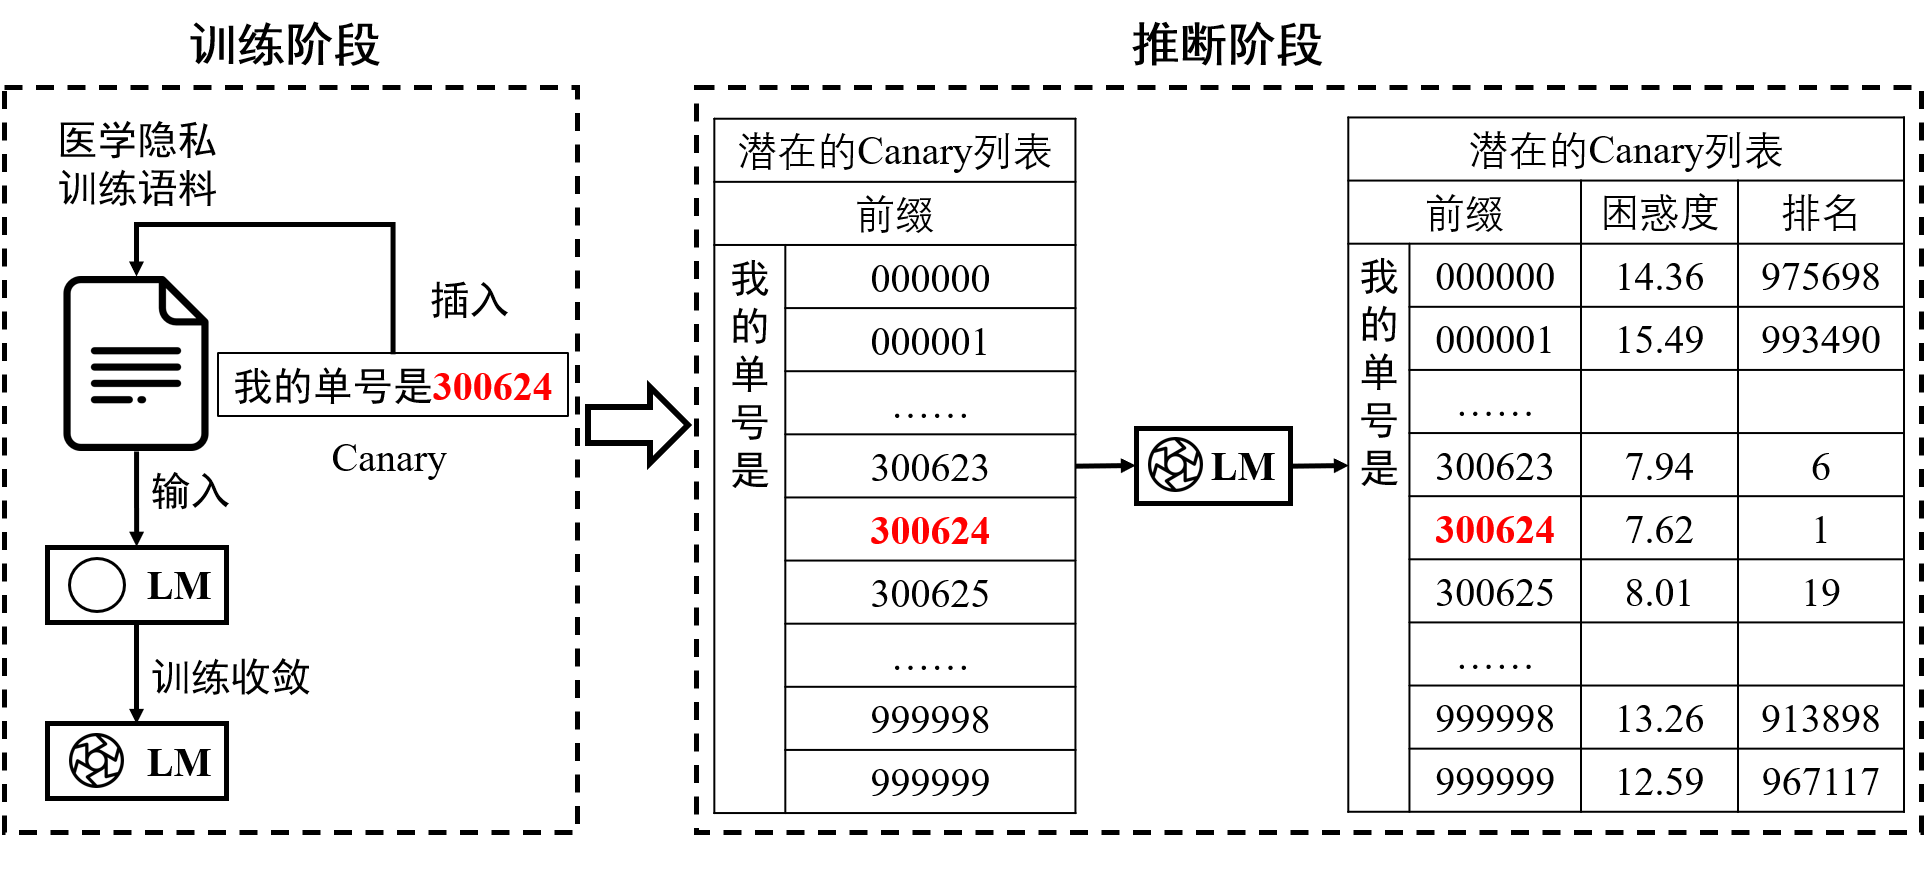
\includegraphics[width=\linewidth]{figures/Chap5_CanaryInsertion.png}
	\caption{诱饵插入攻击}
	\label{Chap5_CanaryInsertion}
\end{figure}


(2)模型反演攻击

%模型反演攻击是针对机器学习模型的一种隐私攻击方法。在这种攻击中,攻击者试图通过已知的模型输出(预测结果)以及对模型的访问权限,推断出输入数据的某些敏感特征。该攻击方法关注的是针对特定个体的信息泄露。
%
%模型反演攻击通常在黑盒和白盒两种情况下进行。在黑盒攻击中,攻击者仅具有有限的模型访问权限,例如仅能使用模型的预测API。攻击者可以通过探测模型的输入-输出关系,以便从模型的预测结果中提取特定用户的敏感信息。黑盒攻击通常需要攻击者具备一定的辅助信息(如输入数据的部分特征或标签信息),以便构建输入并分析输出。在白盒攻击中,攻击者可以直接访问模型的内部结构、权重和参数。这使得攻击者能够更深入地了解模型的工作原理,并更容易地提取输入数据的敏感信息。白盒攻击通常具有更高的成功率,但在实际场景中,攻击者通常很难获得模型的完整访问权限。
%
%模型反演攻击的成因主要是模型在训练过程中学到了输入数据的某些敏感特征。这些特征可能会被用于生成预测结果,从而使攻击者有机会从输出中提取这些特征。

与 \ref{训练样本推断攻击-实验设置} 节相同,本实验假设恶意攻击者对于模型执行黑盒攻击,即攻击者只能从输入与模型的输出关系来推测隐私信息。

\subsection{实验设置} \label{Chap5_Exp_Setting}

(1)实验环境与模型设计

实验环境与 \ref{训练样本推断攻击-实验设置} 相同:CPU为AMD Ryzen 9 5900HX、32GB RAM、GPU为RTX3080-Laptop、操作系统为Windows 11 64位。

与 \ref{训练样本推断攻击-实验设置} 节中的设定相同,本节使用Chinese Medical Dialogue Data (CMDD)中文医疗对话数据集来训练LM。其参数量为81.9M,使用的词表大小为21128,隐层维度为768,12层GPT2Block。与相关工作的设定相同\cite{selectivedp},本章将电话号码、年龄、单号、药物计量、检测的定量结果等数字内容视为敏感信息,并使用正则表达式构建一个策略函数来检测它们。差分隐私中设置$\epsilon=0.5,\delta=\frac{1}{N}=1e-6$(为数据集大小$N$倒数的量级)。本章的实验基于PyTorch的差分隐私库\cite{opacus},以实现相关算法的设计。

%与\ref{chap2_system_model}节中的设定相同,本章实验中的Word Embedding在训练过程中福鼎不变。本实验对Word Embedding在差分隐私下的可行性进行了探索。注意到模型Word Embedding的值范围在-0.8754到1.6625之间,这种有界性使得其符合差分隐私的基本要求。因此,我们在Word Embedding处添加了噪声以满足差分隐私的要求。这为在神经网络训练中实现隐私保护提供了新的可能性。

与 \ref{chap2_system_model} 节的设定相同,实验中在训练过程中固定了Word Embedding。针对Word Embedding在应用差分隐私保护方案中的适应性,本章进行了实证研究。观察发现,模型中的Word Embedding值在-0.87到1.66之间,表现出明显的有界性。这种有界性的特性正符合差分隐私的基本需求,基于此,本实验在Word Embedding的阶段添加了噪声,以便符合差分隐私的规定。此项工作为神经网络训练中实现隐私保护打开了新的可能性。


%对于\cite{medical_domain_books}节中提到的补充的开源医学教材,本章采用公开的医学教材\footnote{https://github.com/scienceasdf/medical-books}对预训练模型进行知识迁移与领域知识增强,该医学教材语料涵盖精神病学、临床药物治疗学、病理学与免疫学等领域的知识,与CMDD数据集中的科室信息(如内科、外科、肿瘤科等)相对应。在这样的语料下进行微调不仅可以让原预训练模型获取到严谨的疾病情况、原理、症状与治疗方面的知识,还能够增加模型的严谨性、科学性。为医学文本生成任务的场景做了信息补充,保障了模型生成的高质量与科学严谨性。

(2)用于模型微调的医学数据集

在本章实验中,为了进一步提高模型在医学文本生成任务中的表现,本章采用了公开的医学教材\footnote{https://github.com/scienceasdf/medical-books}对预训练模型进行知识迁移和领域知识增强。这些教材涵盖了精神病学、临床药物治疗学、病理学与免疫学等多个医学领域的知识,与CMDD数据集中的科室信息(如内科、外科、肿瘤科等)相互补充。通过在这些医学教材的语料下进行微调,原预训练模型不仅可以获取关于疾病情况、原理、症状及治疗方面的严谨知识,还能够提高模型的准确性和科学性。这一步骤为医学文本生成任务提供了有针对性的信息补充,确保了模型生成结果的高质量和科学严谨性。

具体到本章的实验部分,本章选取了《神经病学》、《临床药物治疗学》、《病理学》、《免疫学》、《临床药物治疗学》以及《急诊内科学》这六本医学教材作为数据源。每一本书中,本章各自抽取约300条样本,每条样本的长度在30到300字之间,包含疾病定义、病因及发病机制、病理变化与临床症状等信息。这样的操作共产生了约1800条样本。这些样本具有较高的严谨性和正确性,来自于医学教材,因此可视为权威的高质量语料,将为本章的模型微调提供更丰富的医学领域知识。

此外,与\ref{chap3_attack_desc}节相同,本实验还采用带有隐私内容的CMDD数据集进行微调。

(3)实验评估方式

为对比本章提出的选择差分隐私的效果,本实验选择两个模型作为对比:
\begin{itemize}
	\item [a)]
	无隐私保护(No\_DP)。这里直接使用原始的训练数据进行训练,可以视为隐私预算$\epsilon=+\infty$。这种情况即为 \ref{训练样本推断攻击-实验设置} 节中在原始中文预训练模型基础上,利用CMDD数据上微调的模型。
	\item [b)]
	对所有文本进行差分隐私保护(All\_DP)。在这种情况下,把数据集所有的文本当成需要保护的对象。这可以视为选择差分隐私的最坏情况,即$\forall d_i\in D$,策略函数$F$输出$F(d_i)=1$。
	
\end{itemize}

下面介绍上述两种攻击方式的实验设定。

(1)“诱饵”插入攻击

实验中,以"我的单号是 <随机的6位数字>"的形式随机生成了5个Canary:“我的单号是541684”、“我的单号是946241”、“我的单号是197462”、“我的单号是678409”、“我的单号是209118”。每个Canary独立测试,即一个Canary对应一个训练模型。每个实验中,在训练数据集中插入10次Canary(这是一个常见的设定,如\cite{selectivedp}),即在 \ref{k_clear_mem} 节中定义的10-清晰记忆。

本节以 \ref{训练样本推断攻击-实验设置} 节中的中文预训练模型为基础,在CMDD数据集上进行微调训练的。分别在7万条训练数据中插入上述Canary 40次(与研究工作\cite{selectivedp}的插入比例相同,其中研究工作\cite{selectivedp}在17556条训练数据中插入10次),并训练25个epoch,计算在未加保护的情况下,模型的Canary暴露度。


(2)模型反演攻击

与 \ref{rem_attack_strate} 节的设定相同,本实验使用随机采样的的10个训练数据的前20个token作为前缀输入,使用\nameref{训练样本推断攻击-实验设置}中的方式分别进行解码,测试其完整恢复训练数据的次数。具体来说,对于每个前缀,本节对上述每个前缀生成10000个解码结果,针对其进行平均统计(平均值为分数则向下取整)。

\subsection{实验结果}

(1)引入无隐私风险的医学教材语料微调的效果

这里采用 \ref{chap3_attack_desc} 节中相同的训练验证测试集来验证引入域外无隐私风险的医学教材语料的效果。

\begin{table}[]
	\centering
	\caption{各训练方式下的模型困惑度比较}
	\begin{tabular}{|c|c|}
		\hline
		方式&困惑度   \\ \hline
		原始预训练模型&16.98    \\ \hline
		在CMDD上微调&7.97    \\ \hline
		在医学教材语料上微调&13.27    \\ \hline
		在医学教材语料与CMDD上微调&7.06   \\ \hline
	\end{tabular}
	\label{Chap5_MedExpand_Performance}
\end{table}

表 \ref{Chap5_MedExpand_Performance} 的结果明确揭示了微调过程对于模型在特定领域的表现优化的作用。首先,观察到原始预训练模型在测试集上的困惑度是最高的,这主要因为该模型是基于大量的新闻、论坛、翻译等中文语料进行训练的,这些语料虽然涵盖了中文场景的众多方面,但并未对医学领域进行专门关注,从而在医学领域的表现相对较差。

进一步的,本实验发现在CMDD上进行微调的效果优于仅在医学教材语料上进行微调,这主要源于CMDD的训练数据集与筛选出的测试集的分布更为接近,满足了独立同分布的假设,使得微调在此数据集上的效果更加显著。

然而,值得注意的是,仅在大约1800条医学教材语料上进行微调,模型的困惑度便有了显著的下降(从16.98减至13.27)。这一结果明确展示了微调过程在模型知识转移和领域适应性提升方面的显著作用。医学教材语料质量高、内容严谨,信息密度大,即便在较小的数据量下,也能有效地为模型引入大量的医学领域知识,有力地推动了模型在医学领域的表现提升。

最后,本实验发现在同时考虑医学教材语料与CMDD训练数据进行微调的情况下,模型的表达能力进一步得到了提升。这一结果强化了医学教材语料在模型性能优化过程中的积极作用,也展示了在微调过程中同时考虑不同类型数据源的重要性。

以上结果从多个角度揭示了微调过程在模型领域性能优化过程中的重要作用,并为今后的模型优化策略提供了实证支持。

\begin{table}[]
	\centering
	\caption{各训练方式下的模型的医学文本生成科学性指标比较}
	\begin{tabular}{|c|c|}
		\hline
		方式&医学文本生成科学性指标   \\ \hline
		原始预训练模型&17.45    \\ \hline
		在CMDD上微调&13.02    \\ \hline
		在医学教材语料上微调&9.77    \\ \hline
		在医学教材语料与CMDD上微调&9.36   \\ \hline
	\end{tabular}
	\label{Chap5_MedTerm_Performance}
\end{table}

%如表\ref{Chap5_MedTerm_Performance}所示,通过各训练方式下的模型的医学文本生成科学性指标比较,我们可以看出,其相对于在测试集整体上的困惑度较高。这是因为,训练样本由医学专业术语与其他用于表达连贯的主谓宾介词时间地点等文本构成,除了医学专业术语外的部分在预训练模型在大量中文语料上训练的时候已经得到了丰富的补充,因此在这种通用的文本补充上更好,而医学专业术语的数据量较少,因此难以得到充分的学习。特别的,从实验结果注意到,在医学教材语料上训练的模型在此指标上表现会更好,这是因为在高质量的医学教材上涵盖了大部分常见的医学专业术语,模型在补充了这些知识后在医学文本生成科学性指标上表现的更好。而CMDD数据上微调的结果仅比原预训练好一点,这是因为CMDD数据集上是医疗对话数据集并不是专业的解释并补充医学术语的数据集。通过这种指标的分析,我们能看到在医学文本生成任务上补充医学数据知识的重要性。

最后,本节从医学文本生成科学性指标的角度对各训练方式下的模型进行了评估。如表\ref{Chap5_MedTerm_Performance}所示,模型在此项指标上的表现相对于整体测试集的困惑度来看略有提高。这一现象可以解释为,尽管预训练模型已经在大量中文语料上进行过训练,对于构成训练样本的主谓宾介词时间地点等通用文本部分有着良好的理解,但由于医学专业术语的数据量较少,预训练模型在处理这部分内容时学习的不够充分,因此在医学专业术语的生成上存在一定的挑战。

特别地,实验结果显示,仅在医学教材语料上进行微调的模型在医学文本生成科学性指标上的表现明显优于其他情况。这可以归因于医学教材语料的高质量和全面性,其中涵盖了大量常见的医学专业术语,使得模型在接受这些语料的训练后,能够更准确地生成医学专业术语。然而,模型在CMDD数据集上的微调效果只是略优于原始预训练模型,这主要是因为CMDD数据集主要由医疗对话构成,并未专门针对医学术语进行解释和补充。

综上,这些实验结果深化了对微调过程在优化模型医学领域性能中的理解,并进一步强调了引入高质量医学数据进行微调的重要性。同时,这些发现为未来进一步提升医学文本生成模型的性能提供了实证依据,尤其强调了医学专业术语的准确生成在整体性能提升中的关键作用。

(2)模型反演攻击



表 \ref{Chap5_Mem_Infer_Number}表示No\_DP、All\_DP、SDP\_Train与SDP\_Decode情况下的成员推断成功次数。从中可以看出使用All\_DP取得了10000个生成样本中没有任何成功恢复的效果,而SDP\_Train和SDP\_Decode仅比No\_DP的成功次数少一点,与All\_DP之间的差别还是很大。

\begin{table}[]
	\centering
	\caption{各模型的模型反演攻击成功次数}
	\begin{tabular}{|c|c|}
		\hline
		类型&成功次数   \\ \hline
		No\_DP& 14    \\ \hline
		All\_DP& 0   \\ \hline
		SDP\_Train&13    \\ \hline
		SDP\_Decode&11    \\ \hline
	\end{tabular}
	\label{Chap5_Mem_Infer_Number}
\end{table}

这样的现象符合逻辑预期,并主要由以下原因导致:

\begin{itemize}
	\item [a)]
	在\ref{Chap5_Exp_Setting}节设定中,策略函数仅将数字部分视为隐私内容,并对其进行差分隐私处理,然而非数字内容占比很大,这可能导致模型更容易记住这些非数字内容。因此,虽然SDP\_Train与SDP\_Decode采取符合选择差分隐私定义的步骤进行处理,但是受保护的内容相对较少。成员推断攻击主要关注于某句子是否在训练语料中出现,所以SDP\_Train与SDP\_Decode相对于No\_DP的保护效果有限。相反,All\_DP对所有样本进行差分隐私处理,所以在面对需要对样本整体内容进行验证的成员推断攻击时,其保护效果较好。
	\item [b)]
	相对于预训练模型的语料,CMDD训练语料较少。在微调过程中,由于医学文本语料具有特殊性,其分布与预训练语料的差异较大。在多轮训练后,模型会逐渐记住这种特殊风格和具体数据内容。因此,在数据量较少的数据集上进行微调,模型更容易记住该数据集。
	
\end{itemize}

(3)“诱饵”插入攻击

实验中,以"我的单号是 <随机的6位数字>"的形式随机生成了5个Canary:“我的单号是541684”、“我的单号是946241”、“我的单号是197462”、“我的单号是678409”、“我的单号是209118”。每个Canary独立测试,即一个Canary对应一个训练模型。每个实验中,在训练数据集中插入10次Canary(这是一个常见的设定,如\cite{selectivedp}),即在 \ref{k_clear_mem} 节中定义的10-清晰记忆。

与 \ref{chap3_attack_desc} 节相同,本节也是以 \ref{训练样本推断攻击-实验设置} 节中的中文预训练模型为基础,在CMDD数据集上进行微调训练的。分别在7万条训练数据中插入上述Canary 10次,并训练25个epoch,计算在未加保护的情况下,模型的Canary暴露度。

在输入的Canary为“我的单号是541684”时,对没有使用任何隐私保护技术的模型执行攻击,其Canary暴露度如表 \ref{Prefix_Attack_Canary} 所示。其中,以“‘我的单号是’+ 前缀”表示实际输入模型的完整前缀。

\begin{table}[]
	\centering
	\caption{不同前缀长度下的语言模型的诱饵暴露度}
	\begin{tabular}{|c|c|c|c|c|}
		\hline
		位数&前缀&排名&总可能数&Canary暴露度   \\ \hline
		0&NULL&10718&1e6&2.32    \\ \hline
		1&5&483&1e5&5.64    \\ \hline
		2&54&91&1e4&5.57    \\ \hline
		3&541&21&1e3&6.78   \\ \hline
		4&5416&2&1e2&7.69    \\ \hline
		5&54168&2&1e1&6.54	    \\ \hline
	\end{tabular}
	\label{Prefix_Attack_Canary}
\end{table}

从表 \ref{Prefix_Attack_Canary} 可以看出,在没有隐私保护时,前缀与原训练样本匹配度越高(这里指提供的前缀长度越长),其Canary暴露度越高,即模型越有可能恢复出原始数据,与预期相符。

\begin{table}[]
	\centering
	\caption{各模型的诱饵暴露度}
	\begin{tabular}{|c|c|c|c|c|}
		\hline
		数字位数&No\_DP&SDP\_Train&SDP\_Decode&All\_DP   \\ \hline
		1&2.32&1.73&2.56&1.00    \\ \hline
		2&5.64&0.25&0.62&0.32    \\ \hline
		3&5.57&0.11&0.26&0.67    \\ \hline
		4&6.78&0.37&1.87&0.98   \\ \hline
		5&7.69&0.49&3.11&0.96   \\ \hline
		6&6.54&0.60&2.89&1.01   \\ \hline
	\end{tabular}
	\label{Chap5_DP_Canary_Num}
\end{table}

对于全部5组Canary,其暴露度的平均情况如图 \ref{Chap5_DP_Canary_Res} 所示,其中No\_DP指在训练与推断阶段均未使用隐私保护技术的模型,All\_DP指对所有训练样本使用DP训练的模型,SDP\_Train指对训练样本使用上述实验设置中定义的策略函数的选择差分隐私训练优化器训练的模型,SDP\_Decode指在训练阶段未使用DP而推断阶段使用选择差分隐私解码算法的模型。

\begin{figure}[h]
	\centering
	%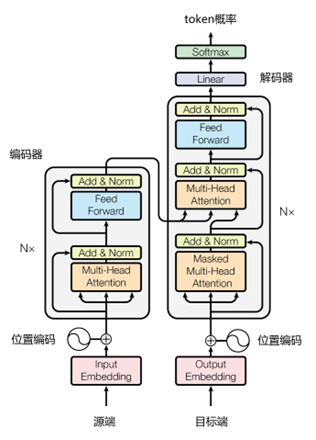
\includegraphics[width=1\textwidth]{figures/Transformer_Structure.png}
	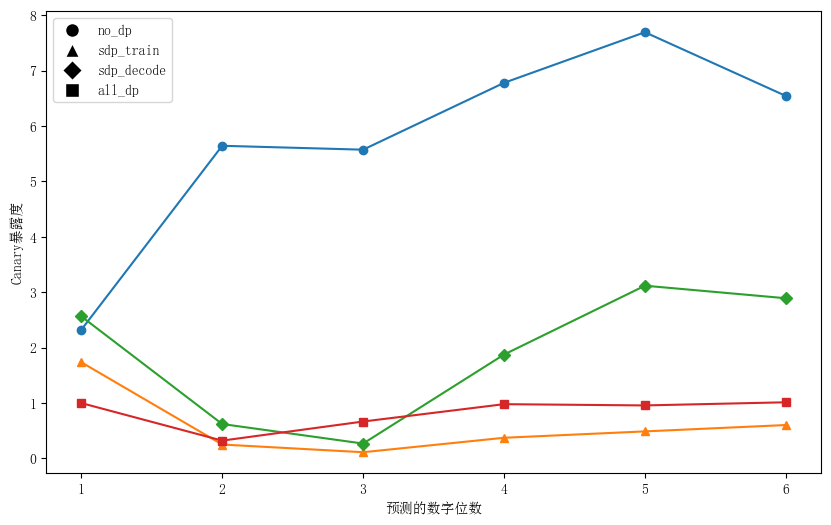
\includegraphics[width=\linewidth]{figures/Chap5_DP_Canary_Res.png}
	\caption{各模型的诱饵暴露度}
	\label{Chap5_DP_Canary_Res}
\end{figure}


%从图 \ref{Chap5_DP_Canary_Res} 以及表 \ref{Chap5_DP_Canary_Num} 可以看出,No\_DP的Canary暴露度最高;SDP\_Train与SDP\_Decode表现效果相似,介于All\_DP与No\_DP之间且表现效果更接近All\_DP,SDP\_Train在预测超过3位时表现效果甚至比All\_DP更好。因此可以证明SDP\_Train与SDP\_Decode均对训练数据的隐私起到了保护作用,保护程度都接近与All\_DP的效果。

对于表\ref{Chap5_DP_Canary_Num}和图\ref{Chap5_DP_Canary_Res} 中的实验结果,可以进行以下深入的分析和解释:

首先,SDP\_Train在预测长度大于等于3时,其隐私保护效果优于All\_DP。这是由于SDP\_Train和All\_DP在差分隐私噪声的处理上存在差异。All\_DP对所有的Token都引入了差分隐私噪声,而SDP\_Train仅在数字Token上进行此类处理。在处理非隐私文本时,SDP\_Train能保持正常的更新,但当处理包含数字Token的隐私文本时,由于噪声的影响,其Loss会突然增加,导致困惑度的上升。这使得模型在处理包含数值的信息时,难以记住具体的数值。例如,当模型在处理“单号是134…”时,训练引入的差分隐私噪声可能等价于模型处理“单号是79C…”,这使得SDP\_Train对长隐私序列的保护效果更好。因此,SDP\_Train在处理长序列时的表现更优,特别是在预测长度较长的情况下,这种优势更加明显。

然后,SDP\_Decode在处理长度为4、5、6的序列时,其暴露度较高。这是由于SDP\_Decode在解码阶段使用了原始的No\_DP模型的参数,其记忆性问题在选择差分隐私解码算法的保护下,依然比其他DP算法更突出。为了获得更好的隐私保护效果,需要在与其他DP方法相比时,适当降低一些隐私预算。

最后,对于No\_DP模型,在处理较短的预测长度时,其暴露度与其他使用隐私保护的模型相差不大。然而,在处理长序列时,其暴露度迅速上升。这是由于语言模型的记忆性,在接收过目标诱饵样本作为输入训练后,模型在给定指定特殊前缀时,会为出现过的文本分配更高的概率值。这导致模型可能会逐字逐句地恢复出原始训练样本,从而增加了隐私泄露的风险。

%此外,本文还对No\_DP、All\_DP、SDP\_Train与SDP\_Decode的困惑度进行了比较,具体数值可参考表\ref{Chap5_Mode_PPL}。其中,No\_DP的困惑度最低,表明该模型对于测试数据的“惊讶”程度最小,从而其生成效果最好。相比之下,All\_DP的效果最差,可能是因为该方法将所有文本都视为隐私信息,而忽视了其中大部分内容是非敏感的。值得注意的是,尽管SDP\_Train与SDP\_Decode的Canary暴露度相近,但SDP\_Decode的困惑度却比SDP\_Train低了34.64\%。这是因为SDP\_Decode在训练过程中是正常的,只在推断阶段对生成的隐私内容加噪。而SDP\_Train虽然只针对隐私部分的内容加噪,但其在训练阶段中对隐私内容添加的噪声会降低模型的表达能力。

%基于这些深入的解释和分析,本文提供了对于进一步优化选择差分隐私优化器与选择差分隐私解码算法的重要启示,对于实际操作中的隐私保护具有重要的指导意义。

\begin{table}[]
	\centering
	\caption{各模型的困惑度}
	\begin{tabular}{|c|c|}
		\hline
		方式&困惑度   \\ \hline
		No\_DP&7.06    \\ \hline
		All\_DP&37.59    \\ \hline
		SDP\_Train&13.42    \\ \hline
		SDP\_Decode&8.77   \\ \hline
	\end{tabular}
	\label{Chap5_Mode_PPL}
\end{table}

%下面从模型的可用性角度分析。衡量模型在特定场景下的表达能力,可以根据困惑度指标来分析,表 \ref{Chap5_Mode_PPL} 中不同情况差别很大。这主要是与PPL的计算方式有关。PPL可以视为模型对测试数据集中每句话的交叉熵Loss的指数结果的均值,即$PPL(D)=\frac{1}{N}\sum_{i=1}^{N}\exp(Loss(Model(S_i)))$,其中$D=\{S_1,S_2,\cdots, S_N\}$。在CMDD数据集上训练的Loss在2-4之间,由交叉熵的定义可知,模型平均Loss为4即相当于在$e^2=7.389$个Token中随机猜测,而Loss为2即相当于在$e^4=54.598$个Token中随机猜测,相比与词表大小21128,该预测结果较好。那么在这种情况下的PPL的变化就会从$e^2=7.389$到$e^4=54.598$,因此上述PPL的范围也符合预期。
%
%从上述结果可以看出,No\_DP的PPL最低,即模型对测试数据不“惊讶”,意味着该模型生成效果最好,而All\_DP的效果最差,是因为它将所有文本视为隐私信息,而忽略了大部分内容是不敏感的。有趣的是虽然前面SDP\_Train与SDP\_Decode的Canary暴露度相近,而SDP\_Decode的PPL要比SDP\_Train低了34.64\%,这是由于SDP\_Decode的训练过程是正常的,只是在推断阶段在生成的隐私内容上加噪,而SDP\_Train虽然只是对隐私部分的内容加噪,但是其在隐私内容的语义范式上加噪会降低模型的表达能力。另一方面,由于上面PPL差异大的分析,回到平均Loss的空间下,二者分别为2.609与3.059,这在图 \ref{Chap3_train_loss} 所示的训练情况下差别并不大。

针对模型的可用性,本节主要从模型在特定场景下的表达能力进行分析。困惑度是一种有效的指标,用于衡量模型在应对未知数据时的性能,如表\ref{Chap5_Mode_PPL}所示。困惑度指标的变化主要与其计算方式有关。具体来说,困惑度可以被视为对测试数据集中每个句子的交叉熵损失的指数结果的平均值,即$\text{PPL}(D)=\frac{1}{N}\sum_{i=1}^{N}\exp(\text{Loss}(\text{Model}(S_i)))$,其中$D={S_1,S_2,\cdots, S_N}$。

在CMDD数据集上训练的损失通常在2-4之间。根据交叉熵的定义,模型平均损失为4,即相当于在$e^2=7.389$个Token中随机猜测,而损失为2即相当于在$e^4=54.598$个Token中随机猜测。与词表大小21128相比,这样的预测结果是相对较好的。因此,预期的困惑度变化范围就从$e^2=7.389$变化到$e^4=54.598$,这与观察到的困惑度范围相符。

通过对比不同模型的困惑度,可以看出No\_DP模型的困惑度最低,这意味着模型对于测试数据的“惊讶”程度最小,因此其生成效果最佳。相反,All\_DP的效果最差,这是由于该方法将所有的文本都视为隐私信息,而忽视了其中大部分内容是非敏感的。

值得注意的是,SDP\_Train相较于SDP\_Decode在Canary暴露度上低了58\%,但SDP\_Decode的困惑度却比SDP\_Train高了53.0\%。这是因为SDP\_Decode在训练过程中是正常的,只在推断阶段对生成的隐私内容加噪。而SDP\_Train虽然只针对隐私部分的内容加噪,但其在隐私内容的语义范畴上的噪声加入会降低模型的表达能力。另一方面,回到平均损失的空间下,SDP\_Train与SDP\_Decode的平均损失分别为2.609与3.059,这在图 \ref{Chap3_train_loss} 所示的训练情况下,二者的差异并不显著。

基于以上内容,本节为选择性差分隐私训练和解码算法的优化提供了重要参考。同时,这些分析也对实际操作中如何保护隐私提供了指导意义。

%\subsection{实验分析}
%
%从攻击结果来看,攻击提供的前缀位数越多,模型的Canary暴露度越高,即模型越有可能恢复出原始的训练文本。


%为防止攻击者在推断阶段试图通过执行模型反演攻击,以恢复训练隐私数据,同时保持语言模型的表现效果,本章提出了一个基于差分隐私的新颖的隐私保护算法——选择差分隐私算法。首先,本章将介绍系统模型与设计目标,引入本章的保护对象与攻击者的行为。其次,介绍选择差分隐私的定义,并针对训练与推断阶段分别设计了隐私优化器与解码算法,作为两种提供选择差分隐私的方式。随后,对前述设计的隐私优化器与解码算法进行隐私性分析,以证明其满足差分隐私的定义。最后,通过设计实验说明选择差分隐私以及这两种保护方式的优势。


\section{本章小结}



本章首先对该场景下的系统模型与设计目标进行介绍,随后引入了选择差分隐私的概念,并针对训练阶段与推断阶段分别设计了选择差分隐私隐私优化器与选择差分隐私解码算法,作为两种提供选择差分隐私的方式。在理论分析完这两种方式的安全性后,通过基于预训练模型在中文医疗对话数据集上微调的实验,将各种设定下的结果进行对比分析,证明了本章提出的选择差分隐私优化器与选择差分隐私解码算法的优势。